\documentclass[submit]{harvardml}

\course{CS181-S22}
\assignment{Assignment \#4}
\duedate{11:59pm EST, March 25, 2022} 

\usepackage[OT1]{fontenc}
\usepackage[colorlinks,citecolor=blue,urlcolor=blue]{hyperref}
\usepackage[pdftex]{graphicx}
\usepackage{graphicx}
\usepackage{caption}
\usepackage{fullpage}
\usepackage{soul}
\usepackage{amsmath}
\usepackage{framed}
\usepackage{amssymb}
\usepackage{color}
\usepackage{todonotes}
\usepackage{listings}
\usepackage{common}

\usepackage[mmddyyyy,hhmmss]{datetime}

\definecolor{verbgray}{gray}{0.9}

\lstnewenvironment{csv}{
  \lstset{backgroundcolor=\color{verbgray},
  frame=single,
  framerule=0pt,
  basicstyle=\ttfamily,
  columns=fullflexible}}{}
 
\begin{document}

\begin{center}
{\Large Homework 4: SVM, Clustering, and Ethics}\\
\end{center}

\subsection*{Introduction}

This homework assignment will have you work with SVMs, 
clustering, and engage with the ethics lecture.  We encourage you to
read Chapters 5 and 6 of the course textbook.

Please submit the \textbf{writeup PDF to the Gradescope assignment `HW4'}. Remember to assign pages for each question.

Please submit your \textbf{\LaTeX\ file and code files to the Gradescope assignment `HW4 - Supplemental'}. 

\newpage

%%%%%%%%%%%%%%%%%%%%%%%%%%%%%%%%%%%%%%%%%%%%%
% Problem 1
%%%%%%%%%%%%%%%%%%%%%%%%%%%%%%%%%%%%%%%%%%%%%
\begin{problem}[Fitting an SVM by hand, 10pts]

  For this problem you will solve an SVM by hand, relying on principled rules and SVM properties. 
  For making plots, however, you are allowed to use a computer or other graphical tools.

Consider a dataset with the following 7 data points each with $x \in \reals$ and $y \in \{ -1, +1 \}$ : \[\{(x_i, y_i)\}_{i = 1}^7 =\{(-3 , +1) , (-2 , +1 ) , (-1,  -1 ), (0, +1), ( 1 , -1 ), ( 2 , +1 ) , (3 , +1 )\}\] Consider
mapping these points to $2$ dimensions using the feature vector $\bphi(x) =  (x, -\frac{8}{3}x^2 + \frac{2}{3}x^4 )$. The hard margin classifier training problem is:
%
\begin{align*}
  &\min_{\mathbf{w}, w_0} \frac{1}{2}\|\mathbf{w}\|_2^2 \label{eq:dcp} \\
  \quad \text{s.t.} \quad & y_i(\mathbf{w}^\top \bphi(x_i) + w_0) \geq 1,~\forall i \in \{1,\ldots, n\}\notag
\end{align*}

Make sure to follow the logical structure of
the questions below when composing your answers, and to justify each step.

\begin{enumerate}
\item Plot the transformed training data in $\reals^2$ and draw the
  optimal decision boundary of the max margin classifier. You can
  determine this by inspection (i.e. by hand, without actually doing
  any calculations).

\item What is the value of the margin achieved by the optimal decision
  boundary found in Part 1?

\item Identify a unit vector that is orthogonal to the decision boundary.

\item Considering the discriminant
  $h(\bphi(x);\boldw,w_0)=\boldw^\top\bphi(x) +w_0$, give an
  expression for {\em all possible} $(\boldw,w_0)$ that define the
  optimal decision boundary from 1.1.  Justify your answer.

  Hint: The boundary is where the discriminant is equal to 0.  Use
  what you know from 1.1 and 1.3 to solve for $\boldw$ in terms of
  $w_0$.  (If you solve this problem in this way, then $w_0$
  corresponds to your free parameter to describe the set of all
  possible $(\boldw,w_0)$.)
  
\item Consider now the training problem for this dataset. Using your
  answers so far, what particular solution to $\boldw$ will be optimal
  for the optimization problem?

\item What is the corresponding optimal value of $w_0$ for the
  $\boldw$ found in Part 5 (use your result from Part 4 as guidance)?
  Substitute in these optimal values and write out the discriminant
  function $h(\bphi(x);\boldw,w_0)$ in terms of the variable $x$ .


\item Which points could possibly be support vectors of the classifier?  Confirm that
  your solution in Part 6 makes the constraints above tight---that is,
  met with equality---for these candidate points.

\item Suppose that we had decided to use a different feature mapping
    $\bphi'(x) = (x, -\frac{31}{12}x^2 + \frac{7}{12}x^4 )$.  Does
    this feature mapping still admit a separable solution?  How does
    its margin compare to the margin in the previous parts?  Based on
    this, which set of features might you prefer and why? 
    
\end{enumerate}

\end{problem}

\subsection*{Solution}

\begin{enumerate}
    \item 
    We have the following $(\phi(x)_1, \phi(x)_2)$ pairs:
    \begin{itemize}
        \item (-3, 30)
        \item (-2, 0)
        \item (-1,-2)
        \item (0,0) 
        \item(1, -2) 
        \item (2,0) 
         \item (3, 30)
    \end{itemize}
    In the plot below, I have shown the optimal decision boundary (in light blue) based off of these points set at $\phi(x)_2 = -1$. The yellow points represent the class $y = 1$ and the dark blue points represent the points $y = -1$.
    
    \begin{figure}
        \centering
        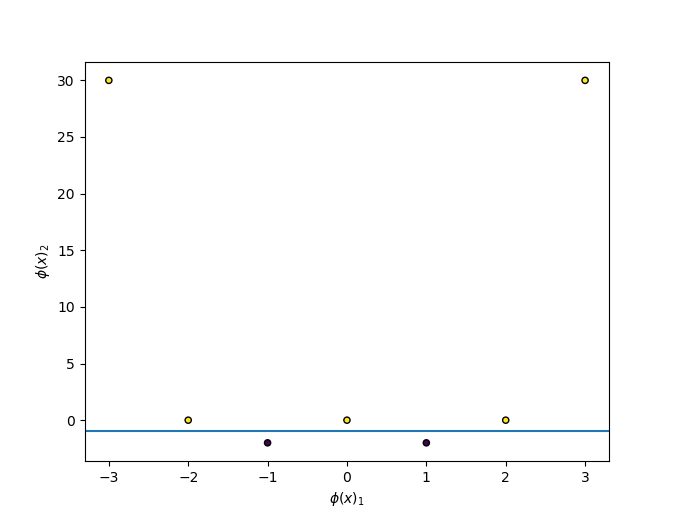
\includegraphics[height=0.4\textheight]{HW4/P1part1plot.png}
    \end{figure}
    
    \item The margin has value of 1.
    \item One unit vector which is orthogonal to the decision boundary is $[\phi(x)_1, \phi(x)_2] = [0, 1]$. 
    \item By inspection, we find that the optimal decision boundary is given by $\phi(x)_2 = -1 \implies \phi(x)_2 + 1 = 0$. \\
    Given the decision boundary form $w^T \phi(x) + w_0 = 0$, it follows that one valid optimal decision boundary is given as $w = [0, 1], w_0 = 1$. \\
    Since scaling $w^T \phi(x) + w_0 = 0$ by some constant will not change our optimal decision boundary, it follows that we can treat $w_0$ itself as our scaling parameter of $w$. \\
    Therefore, all possible parameters describing the optimal decision boundary is given by $w = [0, w_0]$ for $w_0 \in \reals$
    \item Given $y_i(w^T\phi(x_i) + w_0) \geq 1$, we see that the optimal value is given by $w = [0,1]$. 
    \item The corresponding optimal value is $w_0 = 1$. \\
    The discriminant function is then $h(\phi(x); w, w_0)  = [0, 1]^T\phi(x) + 1 = \phi(x)_2 + 1 = - \frac{8}{3}x^2 + \frac{2}{3}x^4 + 1$
    \item For hard margin, support vectors satisfy $y_i h(\phi(x_i); w, w_0) = 1$. It follows that our support vectors are as follows (given in the form $(x_i, y_i)$):
    \begin{itemize}
        \item $(-2,1) \implies (1)h(\phi(-2); w, w_0) = 1(0+1) = 1$
        \item $(-1,-1) \implies (-1)h(\phi(-1); w, w_0) = -1(-2+1) = 1$
        \item $(0,1) \implies (1)h(\phi(0); w, w_0) = 1(0+1) = 1$
        \item $(1,-1) \implies (-1)h(\phi(1); w, w_0) = -1(-2+1) = 1$
        \item $(2,1) \implies (1)h(\phi(2); w, w_0) = 1(0+1) = 1$
    \end{itemize}
    \item  We have the following $(\phi'(x)_1, \phi'(x)_2)$ pairs:
    \begin{itemize}
        \item (-3, 24)
        \item (-2, -1)
        \item (-1,-2)
        \item (0,0) 
        \item(1, -2) 
        \item (2,-1) 
         \item (3, 24)
    \end{itemize}
    In the plot below, I have shown the optimal decision boundary (in light blue) based off of these points set at $\phi(x)_2 = -1.5$. The yellow points represent the class $y = 1$ and the dark blue points represent the points $y = -1$. \\
    We see that this feature mapping still admits a separable solution. However, our margin is now $0.5$, whereas our previous feature mapping had a margin of $1$. Based on this, we would prefer the the first set of feature mappings $phi$ over this new feature mapping $\phi'$. Given that our hard margin classifier is constrained by $y_i (w^T \phi(x_i) + w_0 \geq 1$, it follows that our current training framework will not be able to works optimally towards defining the boundary which perfectly separates our classes using $\phi'$ because we constrain our margin to be larger than the margin which our optimal boundary allows for. Meanwhile, using $\phi$, our margin is equal to the margin for the optimal boundary, so our training framework will be able to work towards optimally finding our ideal decision boundary.

    \begin{figure}
        \centering
        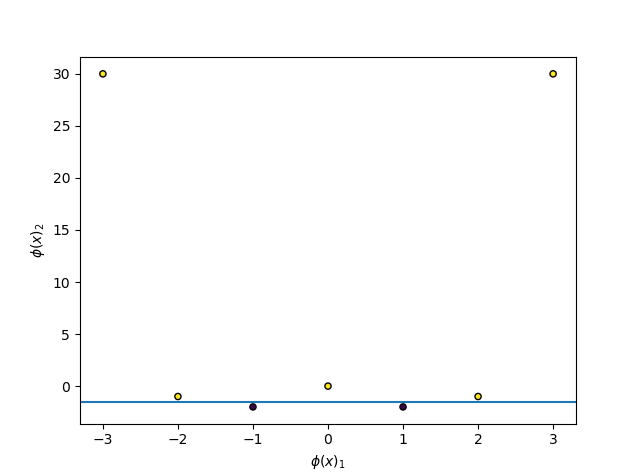
\includegraphics{HW4/P1part8plot.png}
    \end{figure}
\end{enumerate}
%%%%%%%%%%%%%%%%%%%%%%%%%%%%%%%%%%%%%%%%%%%%%
% Problem 2
%%%%%%%%%%%%%%%%%%%%%%%%%%%%%%%%%%%%%%%%%%%%%

\begin{problem}[K-Means and HAC, 20pts]

For this problem you will implement K-Means and HAC from scratch to cluster image data. You may use \texttt{numpy} but no third-party ML implementations (eg. \texttt{scikit-learn}).

We've provided you with a subset of the MNIST dataset, a collection of
handwritten digits used as a benchmark for image recognition (learn more at
\url{http://yann.lecun.com/exdb/mnist/}). MNIST is widely used in supervised learning, and modern algorithms do very well. 

You have been given
representations of MNIST images, each of which is a $784\times1$
greyscale handwritten digit from 0-9. Your job is to implement K-means and HAC on MNIST, and to test whether these relatively
simple algorithms can cluster similar-looking images together.

The code in \texttt{T4\_P2.py} loads the images into your environment into two arrays -- \texttt{large\_dataset}, a 5000x784 array, will be used for K-means, while \texttt{small\_dataset}, a 300x784 array, will be used for HAC. In your code, you should use the $\ell_2$ norm (i.e. Euclidean distance) as your distance metric.

\textbf{Important:} Remember to include all of your plots in your PDF submission!

\textbf{Checking your algorithms:} Instead of an Autograder file, we have provided a similar dataset, \texttt{P2\_Autograder\_Data}, and some visualizations, \texttt{HAC\_visual} and \texttt{KMeans\_visual}, for how K-means and HAC perform on this data. Run your K-means (with $K=10$ and \texttt{np.random.seed(2)}) and HAC on this second dataset to confirm your answers against the provided visualizations. Do \textbf{not} submit the outputs generated from \texttt{P2\_Autograder\_Data}. Load this data with \texttt{data = np.load(`P2\_Autograder\_Data.npy')}.

\begin{enumerate}

\item Starting at a random initialization and $K = 10$, plot the
  K-means objective function (the residual sum of squares) as a
  function of iterations and verify that it never increases.

\item For $K=10$ and for 3 random restarts, print the mean image (aka
  the centroid) for each cluster. There should be 30 total images. Code 
  that creates plots for parts 2, 3, and 4 can be found in \texttt{T4\_P2.py}.

\item Repeat Part 2, but before running K-means, standardize or center
  the data such that each pixel has mean 0 and variance 1 (for any
  pixels with zero variance, simply divide by 1). For $K=10$ and 3
  random restarts, show the mean image (centroid) for each
  cluster. Again, present the 30 total images in a single
  plot. Compare to Part 2: How do the centroids visually differ? Why?

\item Implement HAC for min, max, and centroid-based linkages. Fit
  these models to the \texttt{small\_dataset}.  For each of these 3
  linkage criteria, find the mean image for each cluster when using
  $10$ clusters. Display these images (30 total) on a single plot.

  How do the ``crispness'' of the cluster means and the digits
  represented compare to mean images for k-means?  
  Why do we only ask you to run HAC once?  

  \textbf{Important Note:} For this part ONLY, you may use
  \texttt{scipy}'s \texttt{cdist} function to calculate Euclidean
  distances between every pair of points in two arrays.

\item For each of the HAC linkages, as well as one of the runs of your
  k-means, make a plot of ``Number of images in cluster" (y-axis)
  v. ``Cluster index" (x-axis) reflecting the assignments during the
  phase of the algorithm when there were $K=10$ clusters.

  Intuitively, what do these plots tell you about the difference
  between the clusters produced by the max and min linkage criteria?

  Going back to the previous part: How does this help explain the
  crispness and blurriness of some of the clusters?  
\end{enumerate}
\end{problem}

\newpage
\begin{framed}
\noindent\textbf{Problem 2} (cont.)\\
\begin{enumerate}
\setcounter{enumi}{5}
\item For your K-means with $K = 10$ model and HAC min/max/centroid
  models using $10$ clusters on the \texttt{small\_dataset} images,
  use the \texttt{seaborn} module's \texttt{heatmap} function to plot
  a confusion matrix between each pair of clustering methods.  This
  will produce 6 matrices, one per pair of methods. The cell at the
  $i$th row, $j$th column of your confusion matrix is the number of
  times that an image with the cluster label $j$ of one method has
  cluster $i$ in the second method.  Which HAC is closest to k-means?
  Why might that be?

\item Suppose instead of comparing the different clustering methods to
  each other, we had decided to compute confusions of each clustering
  method to the \emph{true} digit labels (you do \emph{not} have to
  actually compute this).  Do you think how well the clustering match
  the true digits is reasonable evaluation metric for the clustering?
  Explain why or why not.
  
\end{enumerate}
\end{framed}


\subsection*{Solution}

\newpage
%%%%%%%%%%%%%%%%%%%%%%%%%%%%%%%%%%%%%%%%%%%%%
% Problem 3
%%%%%%%%%%%%%%%%%%%%%%%%%%%%%%%%%%%%%%%%%%%%%

\begin{problem}[Ethics Assignment, 5pts]

Select a real-life outcome in Artificial Intelligence or Machine Learning 
that you believe is morally wrong. You can select your own outcome from 
the news or select one of the outcomes in the options below:

\begin{itemize}
    \item COMPAS, a case management tool predicting recidivism that 
        flagged “blacks are almost twice as likely as whites to be 
        labeled a higher risk but not actually re-offend” (Angwin 
        2016).
        
    \item An NLP algorithm filled in the inference “Man is to 
        \_\_\_\_ as woman is to \_\_\_\_” with “Man is 
        to computer programmer as woman is to homemaker” (Bolukbasi 
        et al, 2016).
        
    \item \url{http://www.survivalofthebestfit.com/game}: a game that 
        exemplifies algorithmic bias in resume screening
        
    \item IBM Diversity in faces: insufficient training data for 
        darker-skinned faces
        
    \item Other Unfair Algorithms: Algorithms of Oppression (a really 
        good book with tons of examples), VI-SPDAT, Allegheny Family 
        Screening Tool
        
\end{itemize}
Draw a causal chain that resulted in this outcome and circle the choice points that were the largest contributors to the outcome. At each morally relevant choice point, write two alternative decisions that could have prevented the outcome.

\end{problem}

\subsection*{Solution}
I chose to select the outcome ``An NLP algorithm filled in the inference “Man is to as woman is to ” with “Man is to computer programmer as woman is to homemaker” (Bolukbasi et al, 2016)." \\
Below is my causal chain. I have written two alternative decisions at each morally relevant choice point.
\begin{enumerate}
    \item Google News articles are chosen as input corpus for W2V (word to vector, ie the NLP algorithm of discussion).
    \begin{itemize}
        \item Pre-screen what kind of news articles are chosen. Ensure that no gender-biased news articles are used nor that any gender-biased quotes are referenced in the articles. This would help ensure that the media is working in a 
    \end{itemize}
    \item Words from the news article are turned into vectors by Skip-Gram, an unsupervised learning method where context words are predicted from the target word. We take a two-layer neural network, and encode words from the news article as one-hot vectors of length 300. The rows of the hidden layer weight matrix operates as a look up table for, whose rows are the word vectors (word embeddings) we desire.
    \begin{itemize}
        \item Increase the size of the vector which encodes our vocabulary! Increasing the number of dimensions could allow for the algorithm to have more leeway in determining similarity between input encoded words, and the algorithm could be more specific.  
    \end{itemize}
    \item W2V has similar computed word embeddings (from the hidden layer) for these words to be similar, encompassing similarity between vectors ranging from semantic to syntactic patterns. Cosine vector similarity is used to determine similarity between 
    \begin{itemize}
        \item We should have a framework where there is more cases for the 
    \end{itemize}

\end{enumerate}
\newpage
%%%%%%%%%%%%%%%%%%%%%%%%%%%%%%%%%%%%%%%%%%%%%
% Name and Calibration
%%%%%%%%%%%%%%%%%%%%%%%%%%%%%%%%%%%%%%%%%%%%%
\subsection*{Name}
Arnav Srivastava
\subsection*{Collaborators and Resources}
Whom did you work with, and did you use any resources beyond cs181-textbook and your notes?\\
No partners.
\\
Resources:
\begin{itemize}
    \item https://code.google.com/archive/p/word2vec/
    \item https://arxiv.org/pdf/1607.06520.pdf
    \item https://israelg99.github.io/2017-03-23-Word2Vec-Explained/
\end{itemize}
Did you attend office hours for help with this homework?
No.
\subsection*{Calibration}
Approximately how long did this homework take you to complete (in hours)? 
20
\end{document}